\EnableTitleSlide
\section{Grundlagen}

\begin{frame}{Rewrite Rules}
    \textbf{Benutzen einer Rewrite Rule}: \vspace{5mm}

    \begin{tcbitemize}[raster equal height=rows, raster columns=3,
        raster every box/.style={size=small,valign=center,halign=center,colframe=white,colback=white}]
        \tcbitem
        \tcbitem {\Large\color{red-500} $a \cdot 0 \Leftrightarrow 0$ }
        \tcbitem 
    \end{tcbitemize}\vspace{5mm}
    \pause

    \begin{tcbitemize}[raster equal height=rows, raster columns=3,
        raster every box/.style={size=small,valign=center,halign=center,colframe=white,colback=white}]
        \tcbitem {\Large $x + \eqnmarkbox[red]{node5}{y \cdot 0}$ } 
        \annotate[yshift=-1.5em]{below,right}{node5}{Anwenden der Regel} 
    \tcbitem\begin{tikzpicture}
        \draw[line width=10mm, -{Stealth[length=4mm, open, round]}, black, thick] (0,0) -- (2,0);
    \end{tikzpicture}
        \tcbitem {\Large $x + 0$}
    \end{tcbitemize}
\end{frame}

\begin{frame}{Naiver Algorithmus}

    \begin{algorithm}[H]
        \caption{Naiver Algorithmus zur Optimierung von Ausdrücken}\label{alg:ausdruck1}
        \begin{algorithmic}
          \Function{optimize\_expression}{expression}
          \State rules $\gets$ [\ldots]
          
          \While{old\_expression $\neq$ expression}
            \State old\_expression $\gets$ expression
      
            \For{rule in rules}
              \If{match(expression, rule)}
              \State apply(expression, rule)
              \EndIf
            \EndFor
          \EndWhile
      
          \State \Return expression
          \EndFunction
        \end{algorithmic}
      \end{algorithm}
   
\end{frame}

\begin{frame}{Phase Ordering Problem}
    \begin{center}
        \textbf{Welche Regel soll zuerst angewendet werden?}
    \end{center}\vspace{5mm}

    \begin{center}
        {\Large $\left(\eqnmarkbox[red]{node5}{\frac{x \cdot 2}{2}} + x \cdot \frac{y - 3 + 3 + z \cdot 0}{x}\right)^2$ }\vspace{7mm}
    \end{center}

    \begin{center}
        \textbf{Mögliche Resultate:}
    \end{center}\vspace{2mm}

    \begin{tcbitemize}[raster equal height=rows, raster columns=2,
        raster every box/.style={size=small,valign=center,halign=center,colframe=white,colback=white}]
        \tcbitem {\Large $\eqnmarkbox[red]{node5}{\frac{x \ll 1}{2}}$}
        \tcbitem {\Large $\eqnmarkbox[red]{node5}{x}$}
    \end{tcbitemize}
\end{frame}

\begin{frame}{Lösung}
    \textbf{Speichern aller möglichen Ausdrücke in Liste}: \vspace{5mm}

    \begin{tcolorbox}[title=ExprList, center title]
        $\left(\eqnmarkbox[red]{node5}{\frac{x \cdot 2}{2}} + x \cdot \frac{y - 3 + 3 + z \cdot 0}{x}\right)^2$,
        $\left(\eqnmarkbox[red]{node5}{\frac{x \ll 1}{2}} + x \cdot \frac{y - 3 + 3 + z \cdot 0}{x}\right)^2$,
        $\left(\eqnmarkbox[red]{node5}{x} + x \cdot \frac{y - 3 + 3 + z \cdot 0}{x}\right)^2$
    \end{tcolorbox}
\end{frame}

\begin{frame}{Verbesserung}
    \textbf{Sharing und Klassen}: \vspace{5mm}

    {\captionsetup[figure]{oneside,margin={0.4cm,0cm}}
\begin{minipage}[c]{0.49\textwidth}
    \begin{figure}[H]
        \centering
        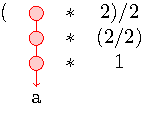
\includegraphics[scale=1.6]{utils/sharing.pdf}
        \caption{Sharing bei einer Liste von Ausdrücken}
        \label{fig:sharing}
    \end{figure}
    \end{minipage}
    \begin{minipage}[c]{0.49\textwidth}
    \begin{figure}[H]
        \centering
        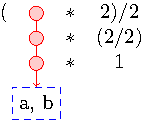
\includegraphics[scale=1.6]{utils/classes.pdf}
        \caption{Kombination aus Sharing und Klassen bei einer Liste von Ausdrücken}
        \label{fig:classes}
    \end{figure}
\end{minipage}}
\end{frame}

\begin{frame}{E-Graphs (1)}
    \begin{figure}[H]
        \centering
        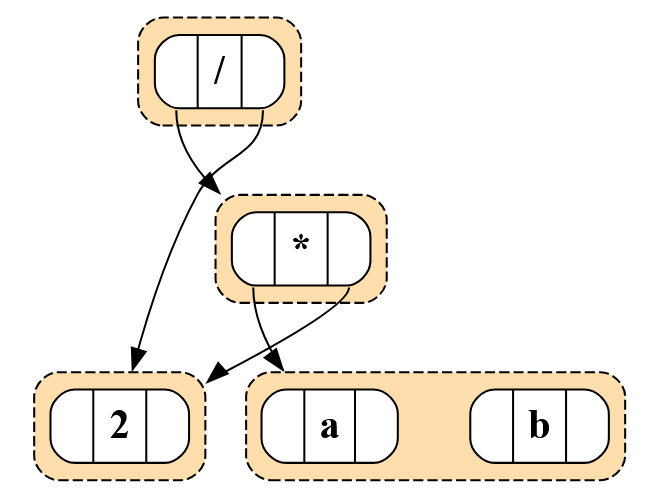
\includegraphics[scale=0.4]{utils/egraph_exp.png}
        \caption{Beispiel eines E-Graphs, der die Ausdrücke $(a \cdot 2) / 2$ und $(b \cdot 2) / 2$ enthält}
        \label{fig:egraphexp}
    \end{figure}
\end{frame}

\begin{frame}{E-Graphs (2)}
Der \textit{E-Graph} als Datenstruktur für Abbildung~\ref{fig:egraphexp}: \vspace{5mm}

\begin{itemize}
\setlength\itemsep{1em}
  \item $\mathbf{U}$: \{ID1\}, \;\; \{ID2\}, \;\; \{ID3\}, \;\; \{ID4, ID5\} 
  \item $\mathbf{M}$: \\ $ID1 \rightarrow EClass(\ldots)$, \\ $ID2 \rightarrow EClass(\ldots)$, \\ $ID3 \rightarrow EClass(\ldots)$, \ldots 
  \item $\mathbf{H}$: \\ $/ \rightarrow ID1$, \\ $* \rightarrow ID2$, \\ $2 \rightarrow ID3$, \\ $a \rightarrow ID4$, \\ $b \rightarrow ID5$
\end{itemize}
\end{frame}

\begin{frame}{Equality Saturation}
    \begin{algorithm}[H]
        \caption{Traditioneller Equality Saturation Workflow nach~\cite{2021-egg}}\label{alg:eqsat} % \cite{2021-egg} ~\footcite{2021-egg}
        \begin{algorithmic}
          \Function{eqsat}{expr, rewrites}
          \State egraph $\gets$ initial\_egraph(expr)
            
          \While{$\mathbf{not}$ egraph.is\_saturated\_or\_timeout()}
            
            \For{rw in rewrites}
              \For{(subst, eclass) $\mathbf{in}$ egraph.ematch(rw.lhs)}
                \State  eclass2 $\gets$ egraph.add(rw.rhs.subst(subst))
                \State egraph.merge(eclass, eclass2)
              \EndFor 
            \EndFor
          \EndWhile
      
          \State \Return egraph.extract\_best()
          \EndFunction
        \end{algorithmic}
    \end{algorithm}
\end{frame}